\chapter{Frequency response and the Bode plot}\label{chap:freqresp}

In this lab you will examine the relationship between the impulse response,
the transfer function, and the frequency response.  You will also compute the
Bode (pronounced ``Boh-dee'') plot of the open-loop motor scheme depicted in
Figure~\ref{fig:openLoop2}\@.
\begin{figure}[htbp]
\centering
\begin{picture}(210,50)
\put(0,20){\(\hat{u}(s)\)}
\put(20,23){\vector(1,0){30}}
\put(55,6.5){\framebox(85,35){\Large\(\frac{k_{E}}{s(s+\frac{1}{\tau})}\)}}
\put(142,23){\vector(1,0){30}}
\put(176,20){\(\hat{\theta}(s)\)}
\end{picture}
\caption{Open-loop motor schematic in frequency domain}\label{fig:openLoop2}
\end{figure}%

\section{Key Concepts}
In this lab we will be determining the relationship between the inputs and outputs 
of a system. Here are a few key topics:
\begin{enumerate}
\item The \emph{Dynamics} of a system govern the input/output relationship
 of a system. These dynamics can be either known, or unknown. In lab~\ref{chap:intro}, 
we observed how our system responded to a simple constant input, however we wish to know 
how it will respond to \emph{all} functions. This is done by observing what is called the 
``Frequency Response" of the system.
\item The  frequency response of a system is determined by first constructing a Bode Plot.  
This is done by inputting different sine waves with varying frequencies, and measuring 
the magnitude and phase difference between the input and the output. For example, 
Figure~\ref{fig:FreqResp} shows the input and output of the system for a sine wave with 
$\omega_u = 5$ rads/sec. Notice how the  magnitude of the output is larger, and the peak time
is shifted by roughly 0.05s. This observation will be made for sine waves with frequencies varying 
from 0.5 rads/sec to 300 rads/sec, or possibly even higher. 
\begin{figure}[htbp]
\centering
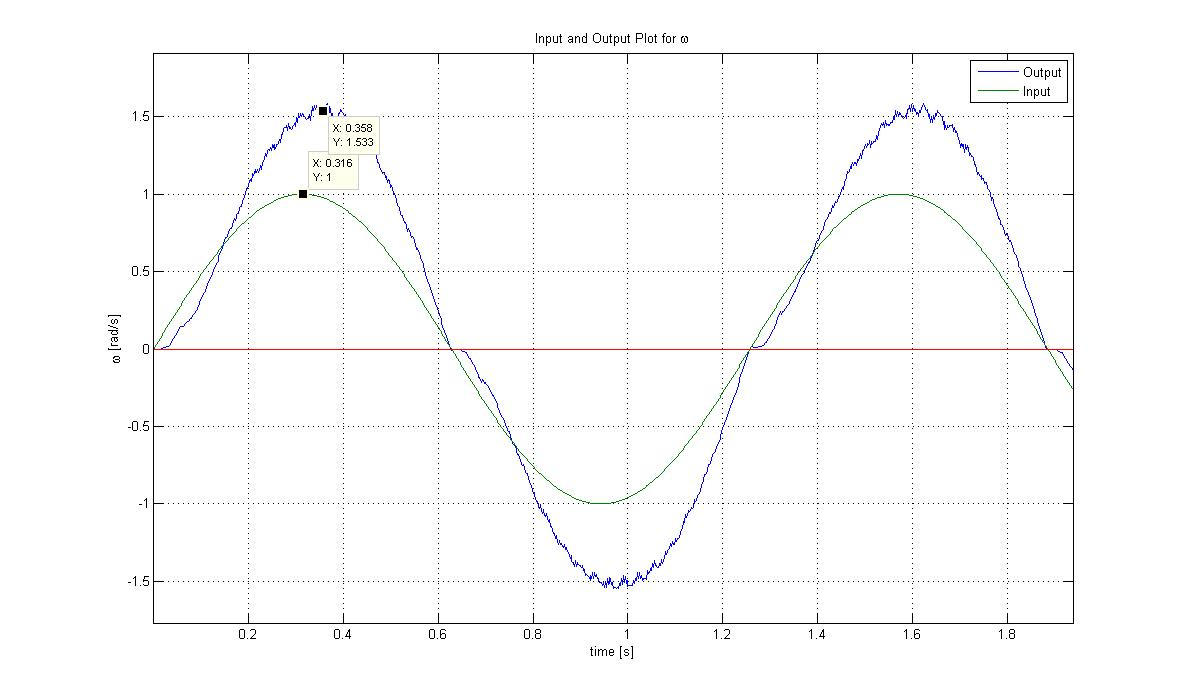
\includegraphics[width=\hsize,height = 0.6\hsize]{pix/FreqResp.jpg}
\caption{\textsf{Matlab} generated plot of the input and output  of the system for $\omega_u = 5$ rads/sec}\label{fig:FreqResp}
\end{figure}

\item Once we have  sufficient data for the magnitude and phase difference, two plots will be created 
(frequency vs. magnitude, and frequency vs. phase angle) using a logarithmic scale. These are your Bode Plots. %reword
\item It is important to remember how these relationships relate to Figure~\ref{Process}. 
In this lab we are conducting experiments as if we did not already know the dynamics of the system. 
This will be how you determine the frequency response of the system you are given for your project,
which will allow you to find a model transfer function for the ``Plant".  


\end{enumerate}

\section{Prelab}\label{sec:prelab4}

\begin{enumerate}
\item Please review Sections 4.1, 4.2, and 4.3 of the course notes for relevant on frequency
response and the production of Bode plots.
\item Compute the Bode plot (by hand) of the motor system when the output is
the motor angle $\theta$.  Recall that the transfer function of that system
is
\begin{equation*}
T(s) =\frac{k_{E}}{s(s+\frac{1}{\tau})}.
\end{equation*}
Use the motor time constant, $\tau$, and the torque constant, $k_{E}$\@,
obtained in Lab~\ref{chap:intro}\@.  Please consult with your TA to make sure
you have the correct values.
\item Repeat the above step when the output is motor velocity $\omega$.
Recall that the transfer function of that system is
\begin{equation*}
T(s) =\frac{k_{E}}{(s+\frac{1}{\tau})}.
\end{equation*}
\end{enumerate}

\section{Procedure}

\subsection{Preliminaries}

In this lab you will be gathering data that will be used to construct the
Bode plot.  Determining the magnitude of the output is straightforward, but
the phase between the input and the output sinusoids is somewhat more
troublesome, but still no match for the wits of seasoned veterans of the
Apple Math program.

To determine the phase difference between two sinusoids, we need to compare
two equivalent points on each sinusoid. Convenient points to consider are
peaks of each sinusoid or where each sinusoid is zero.  Since the magnitude
of each sinusoid can differ, it is more convenient to compare where each
sinusoid is zero. From your plot, measure the time difference between when
the input sinusoid is zero and when the output sinusoid is zero.  Knowing the
time difference and the frequency of the sinusoids, you can use the fact that
$\omega=\frac{d\theta}{dt}=\frac{\Delta\theta}{\Delta t}$ to calculate the
phase difference as $\Delta\theta=\omega\Delta t$\@.

You will find that a good way to organize your data is in a table of the
following format:

\begin{table}[htbp]
\centering
\begin{tabular}{|c|c|c|c|c|c|}\hline
$\omega$&Magnitude&Gain (dB)&Zero-Time Difference&
Phase (rad)&Phase(deg)\\\hline
&&&&&\\
&&&&&\\
&&&&&\\
&&&&&\\
&&&&&\\
\hline

\end{tabular}
\caption{Data collection table}
\label{tab:Data}
\end{table}%



\subsection{MATLAB}

In this part of the lab you will use \textsf{Matlab} to produce the Bode
plots of the mathematical model of the system.

\begin{enumerate}
\item Start \textsf{Matlab} and enter the transfer function corresponding to
each output.  Use the \verb|tf| command to generate the transfer function in
the \textsf{Matlab} command window, then produce the Bode plots of each
transfer function using the \verb|bode| command.

Please refer to Appendix~\ref{chap:MATLAB} on how to use the
\verb|tf| and \verb|bode| command in \textsf{Matlab}.
\item Do not print these plots, but do not close \textsf{Matlab} either.
\end{enumerate}

\subsection{Bode plot}

We will now turn our attention to constructing the Bode plot experimentally,
which we will accomplish by examining the output of the motor given a
periodic input.  The frequency response of a system determines how that
system responds to a harmonic input of frequency $\omega_u$\@.  For this lab,
we will take our harmonic input to be the simple sinusoid $\sin(\omega_u t)$\@.

From your work in Section~\ref{sec:prelab4}, you might guess that
constructing a Bode plot for the motor when the output is the motor angle
will be rather difficult, in which case you would be correct.  However, we
will have a quick look at the angular response of the motor to see if it is
consistent with the Bode plot produced in \textsf{Matlab}.

\begin{enumerate}
\item We begin our exploration of the frequency response with a crude
experiment.  We would like to see what happens over a large range of
frequencies, so we would like $\omega_u$ to increase as $t$ increases.  A
simple way to do this is to define the input function to be $5\sin(t^{2})$\@.
\item Follow Figure~\ref{fig:model4} and build a \textsf{Simulink} model to
implement this signal. \emph{Alternatively, you can modify your model from lab 1}.
\begin{figure}[htbp]
\centering
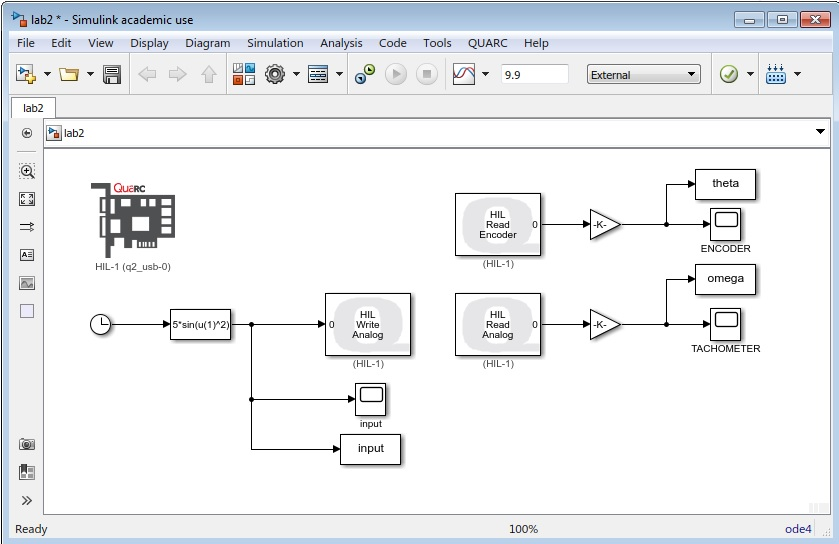
\includegraphics[width=0.6\hsize]{pix/lab2.jpg}
\caption{\textsf{Simulink} model for the implementation of the signal $5\sin(t^{2})$}\label{fig:model4}
\end{figure}%
The \verb|Fcn| block can be found in \textsf{Simulink} in the
\verb|User-Defined Functions| section.  Double-click on your \verb|Fcn| block
to enter the function \verb|5*sin(u(1)^(2))| where \verb|u(1)| represents the
time.  The time is obtained by introducing the \verb|Clock| block as an input
to the function.  The output of the function block is simply connected to the
\verb|Write Analog| block.  Do not forget to change the \verb|solver| to
\verb|ode 4| in \verb|Configuration Paramemters| (\verb|Ctrl+E|). Also,
change the gain constants to the desired units, as in
Step~\ref{enum:parameters} from Lab~\ref{chap:intro}\@. Note: these values can be found in 
Table~\ref{tab:conversionFactors} in Appendix~\ref{chap:hardware}.
\item Change the simulation time in the toolbar to $9.9$~seconds and press enter.
\item \label{enum:simulatet2} Build and run the \textsf{Simulink} model.
Plot the input function $u$, and the output $\theta$ \emph{simultaneously}.
You will notice that $\theta$ is not as well behaved as you might like, but
all you should be concerned with is a rough guess of relative magnitude and
phase with respect to the input function $u$\@.  Does this concur with the
Bode plot you computed with \textsf{Matlab}?  Specifically, comment on the
magnitude and the phase at low and high frequencies.

\item Repeat Step~\ref{enum:simulatet2} but plot the output variable
$\dot\theta$ and $u$ instead of $\theta$ and $u$\@.

\item We will now systematically construct the Bode plot of the motor when
the output is the angular velocity $\omega$ using experimental data. Doing so
will require information about the magnitude and phase of output sinusoid at
various frequencies.  To do this you replace the \verb|Clock| and \verb|Fcn|
blocks by a \verb|Sine Wave| Block.  After you have connected the
\verb|Sine Wave| block to the \verb|Write Analog| block, you can enter the
parameters of the sinusoid you would like to implement.  For the generic
signal, $\sin(\omega_u t)$\@, you may enter the parameters as highlighted in
Figure~\ref{fig:sineConfig}\@.
\begin{figure}[htbp]
\centering
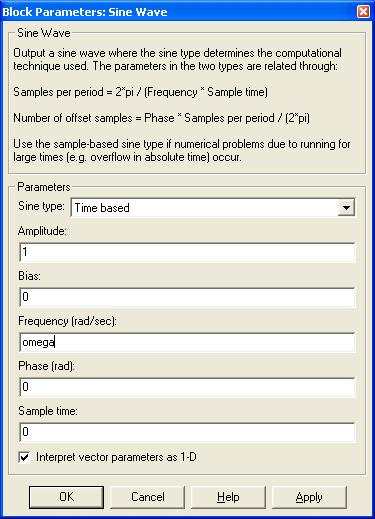
\includegraphics{pix/freqResponseSineConfig.jpg}
\caption{Configuration for the implementation of the signal
$\sin{\omega_u t}$}\label{fig:sineConfig}
\end{figure}%
In this case, the variable \verb|omega|, is undetermined.  The value of
$\omega_u$ must be specified at the \textsf{Matlab} command line before each
run.  The amplitude of $u$ should be set to 1.

\item Build the \textsf{Simulink} model.  For various values of $\omega_u$, run
the system and plot the output variable, $\dot\theta$\@, and the input
variable, $u$\@.  A ``good'' Bode plot can be created using 10--15 well
chosen $\omega_u$ values.  Use the Bode plot generated using \verb|tf| to pick
proper omega values. Note that you do not need to rebuild the \textsf{Simulink} 
model for each new value of $\omega_u$. A good range of $\omega_u$ values would 
be between 0.5 and 300, keeping in mind that this is plotted on a logarithmic scale.%

\item Determine the magnitude of the output sinusoid by recording its peak
amplitude.  It is recommended that you zoom in and out as needed, to ensure a
reasonable degree of accuracy.

\item To determine the phase difference, you will find it most accurate to
look for zero-crossings, as explained above.  You will find that creating an
output variable set to zero is a helpful visual aid in find zero crossings.
Zoom in to accurately observe the time difference when $u$ is zero and when
$\dot\theta$ is zero.  When you are recording the phase differences, you
should be careful that you are recording zero-crossings when both functions are either
increasing or decreasing. This is crucial to keep in mind for higher frequencies.
 This procedure might sound confusing, but usually it is straightforward.%

\item Calculate the phase difference as described in the introduction.

\item With a reasonable amount of data, plot by hand the Bode plot of the
motor when the output is angular velocity, $\omega$. You could also use a
spreadsheet program to organize and plot your data.

When you have completed the lab, make sure you save your files in the folder
you created in the Lab~\ref{chap:intro}\@.
\end{enumerate}

\section{Deliverables}

Prepare a brief write up describing what you learned from this lab. This does not
need to be a formal report, but all material should be presented in a clear and logical manner,
with concise descriptions where necessary. Include the following / answer the following questions:
\begin{enumerate}
\item Include the Matlab generated bode plots for $\theta$ and $\omega$. Use your $k_E$ and $\tau$ values
from lab 1
\item Plots of your motor angular position and velocity compared to the input function $u =  5\sin(t^2)$ (do this on the \emph{same} plot).
Comment on the general trend of the magnitude and phase shift of the outputs. Does this agree
with the bode plots you generated?
\item Include tabulated data from Table~\ref{tab:Data}
\item Include experimental bode plots for both magnitude and phase difference. Ensure the plots \emph{look} like Bode Plots.
\end{enumerate}

%%% Local Variables: 
%%% mode: latex
%%% TeX-master: "lab-manual"
%%% End: 
